This section extends the simulation analysis.

\begin{figure}
\centering
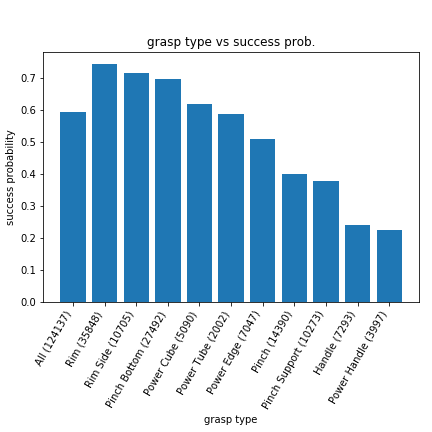
\includegraphics[width=0.8\columnwidth]{images/post-analysis/[2] Grasp_type_vs_success_prob.png}
\caption{Grasp type vs. success probability.}
\label{fig:post2}
\end{figure}

\begin{figure}
\centering
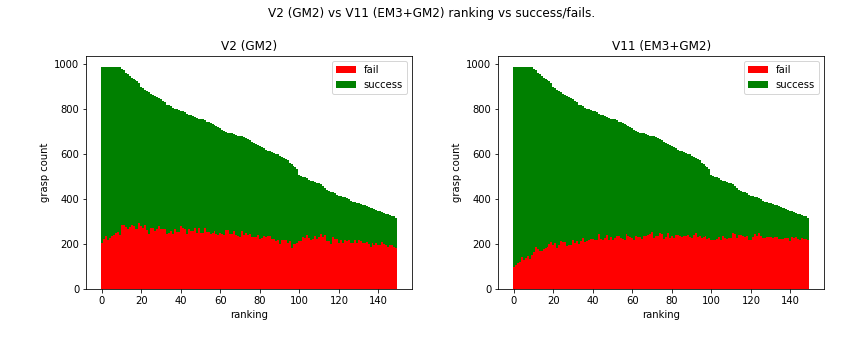
\includegraphics[width=0.8\columnwidth]{images/post-analysis/[3] V2_vs_V11_ranking_vs_success_fail.png}
\caption{Comparison of successful (green) and unsuccessful (red) grasps per ranking for V2 and V11.}
\label{fig:post3}
\end{figure}

\begin{figure}
\centering
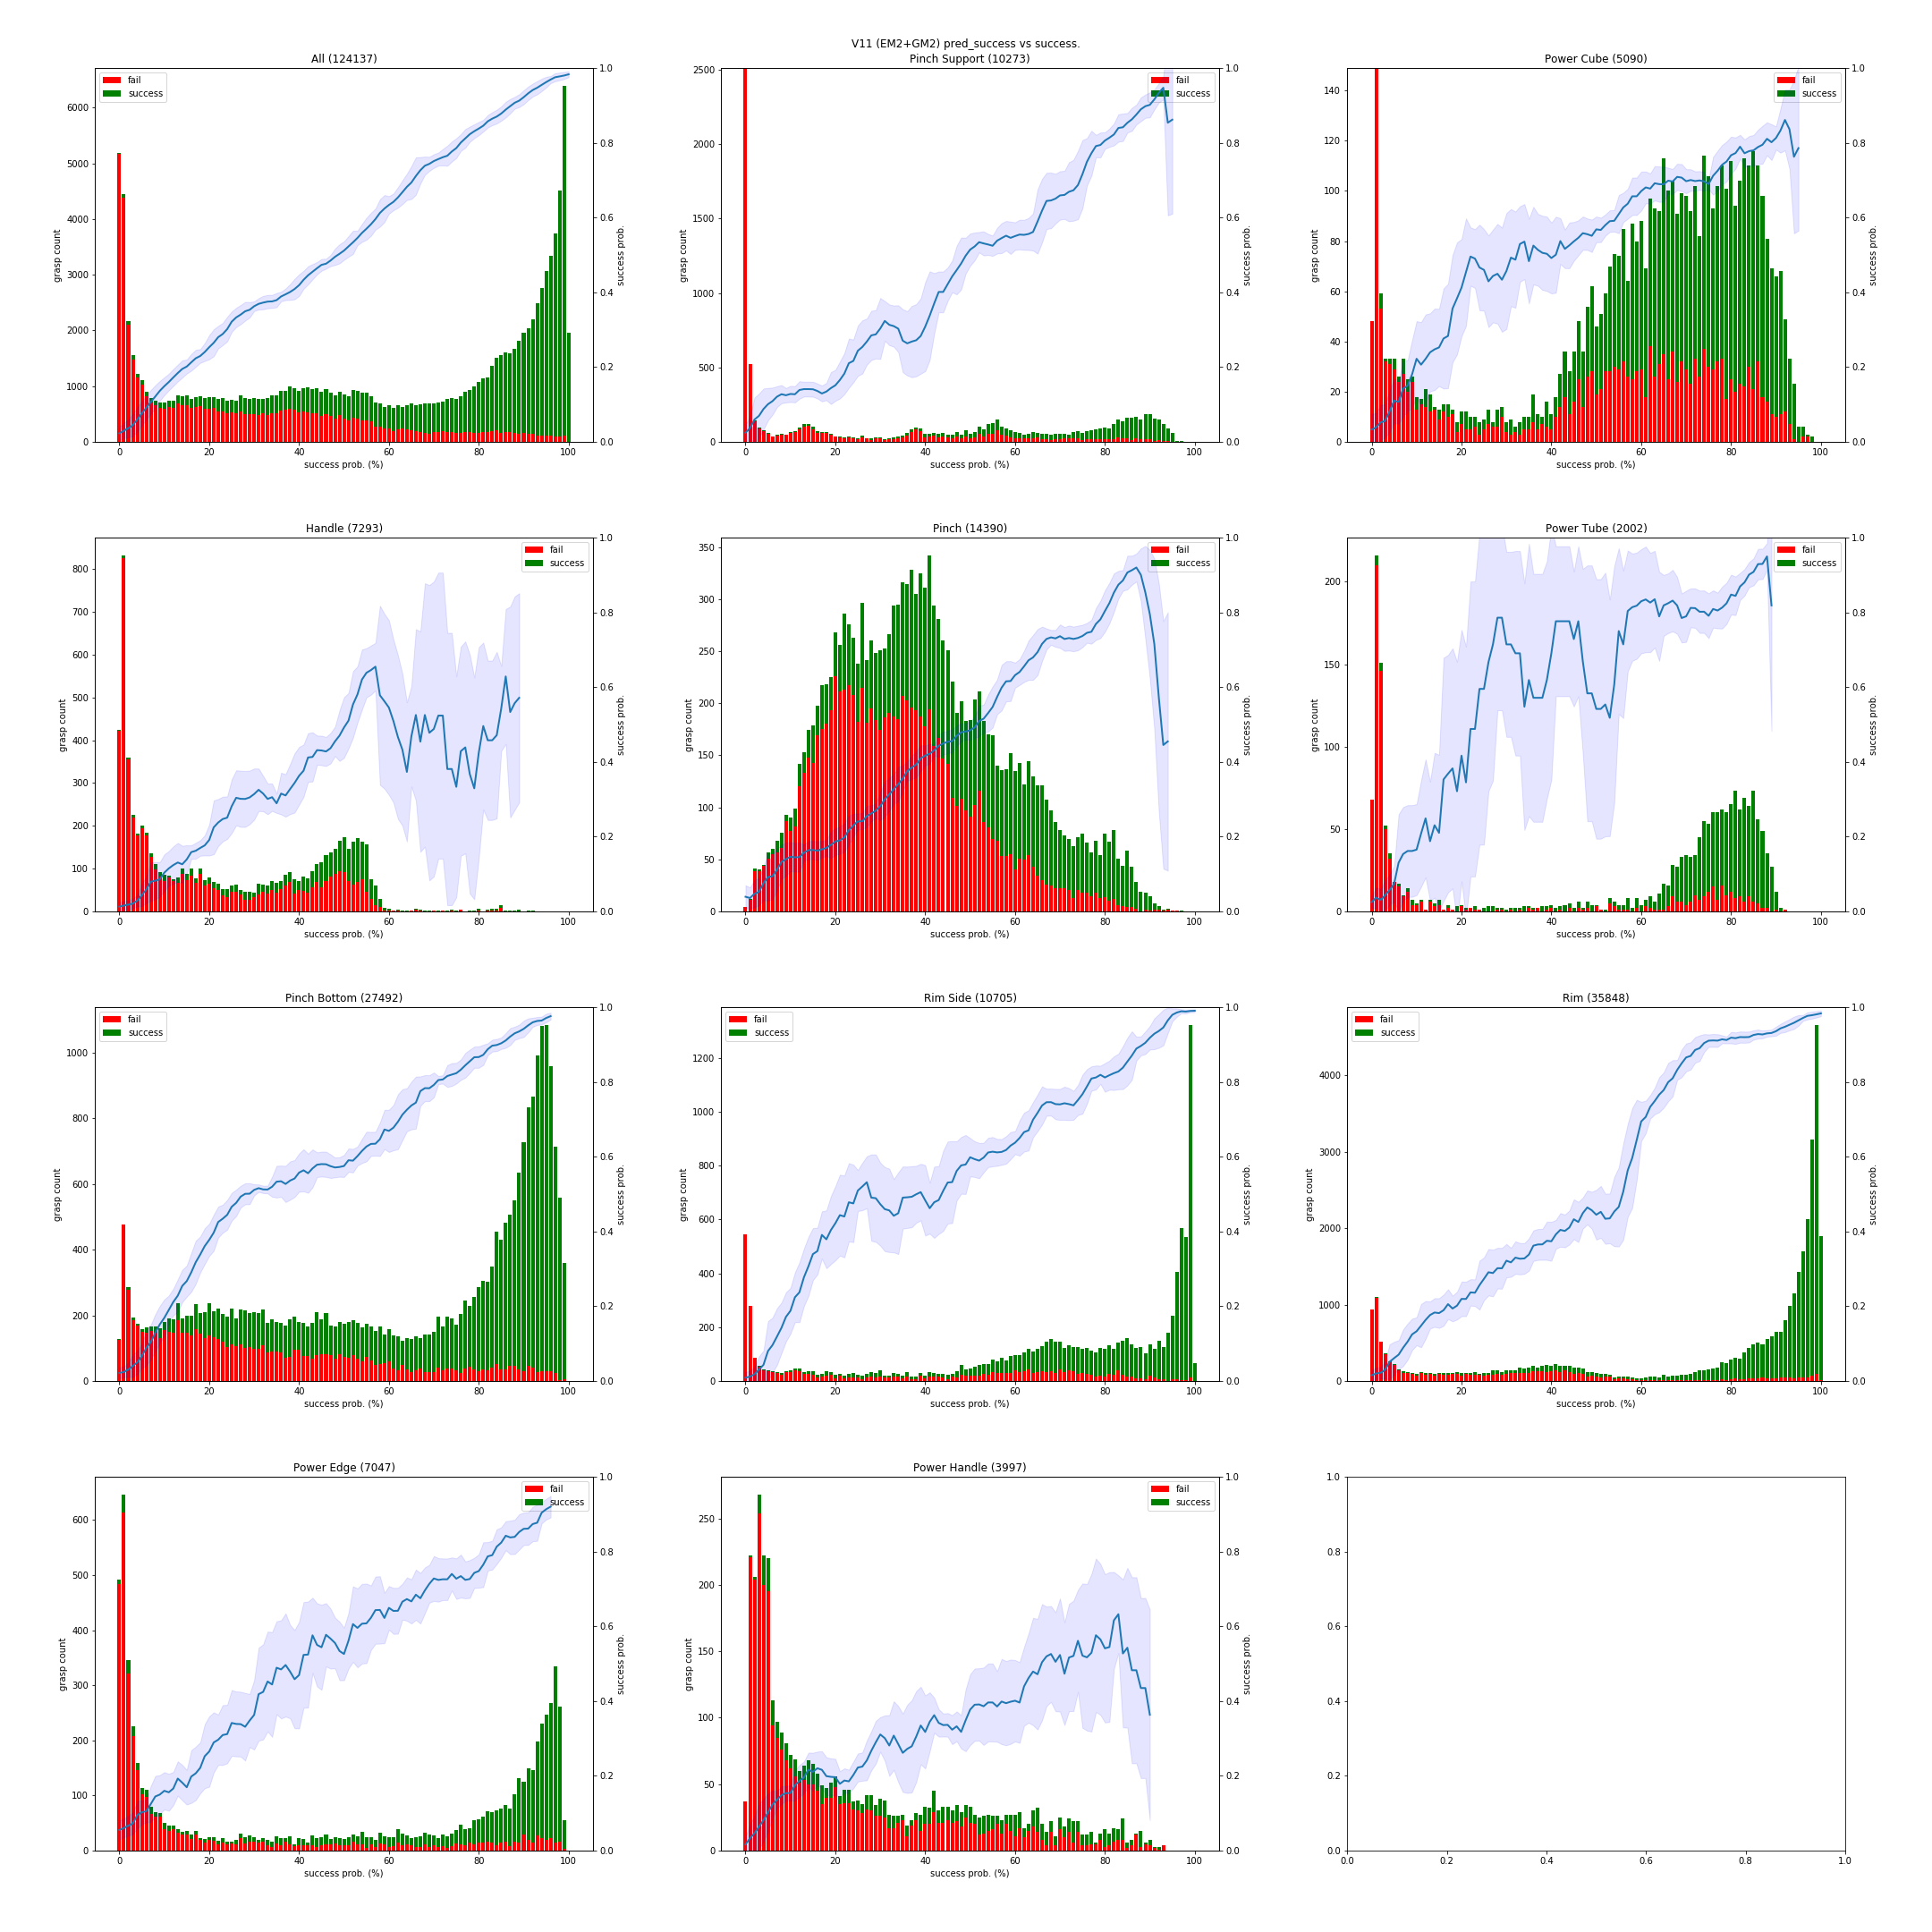
\includegraphics[width=0.8\columnwidth]{images/post-analysis/[4] V11_pred_success_vs_success.png}
\caption{Predicted success probability vs actual success probability for V11.}
\label{fig:post4}
\end{figure}

\begin{figure}
\centering
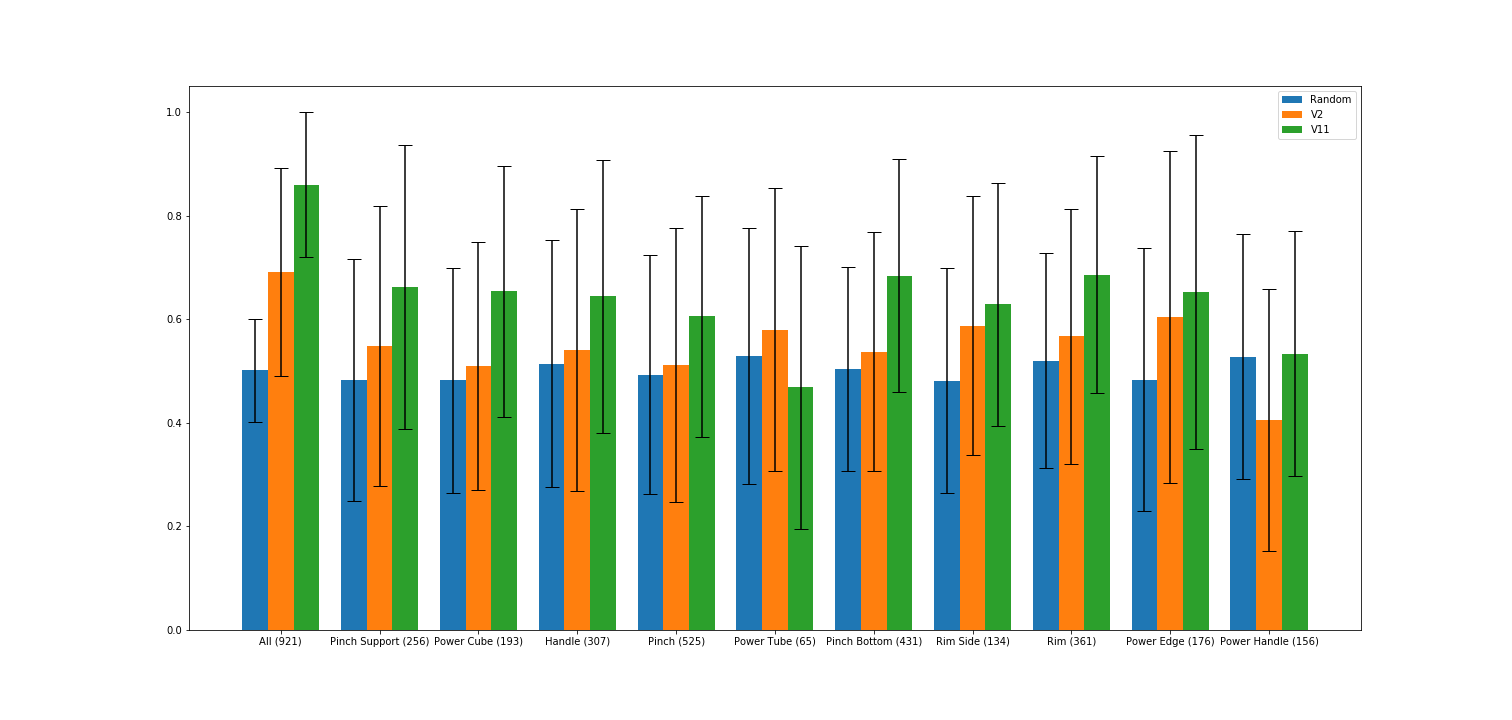
\includegraphics[width=0.8\columnwidth]{images/post-analysis/[5] Ranking_quality_mean_AUC.png}
\caption{Grasp ranking quality comparison of random ranking, V2 and V11.}
\label{fig:post5}
\end{figure}

\begin{figure}
\centering
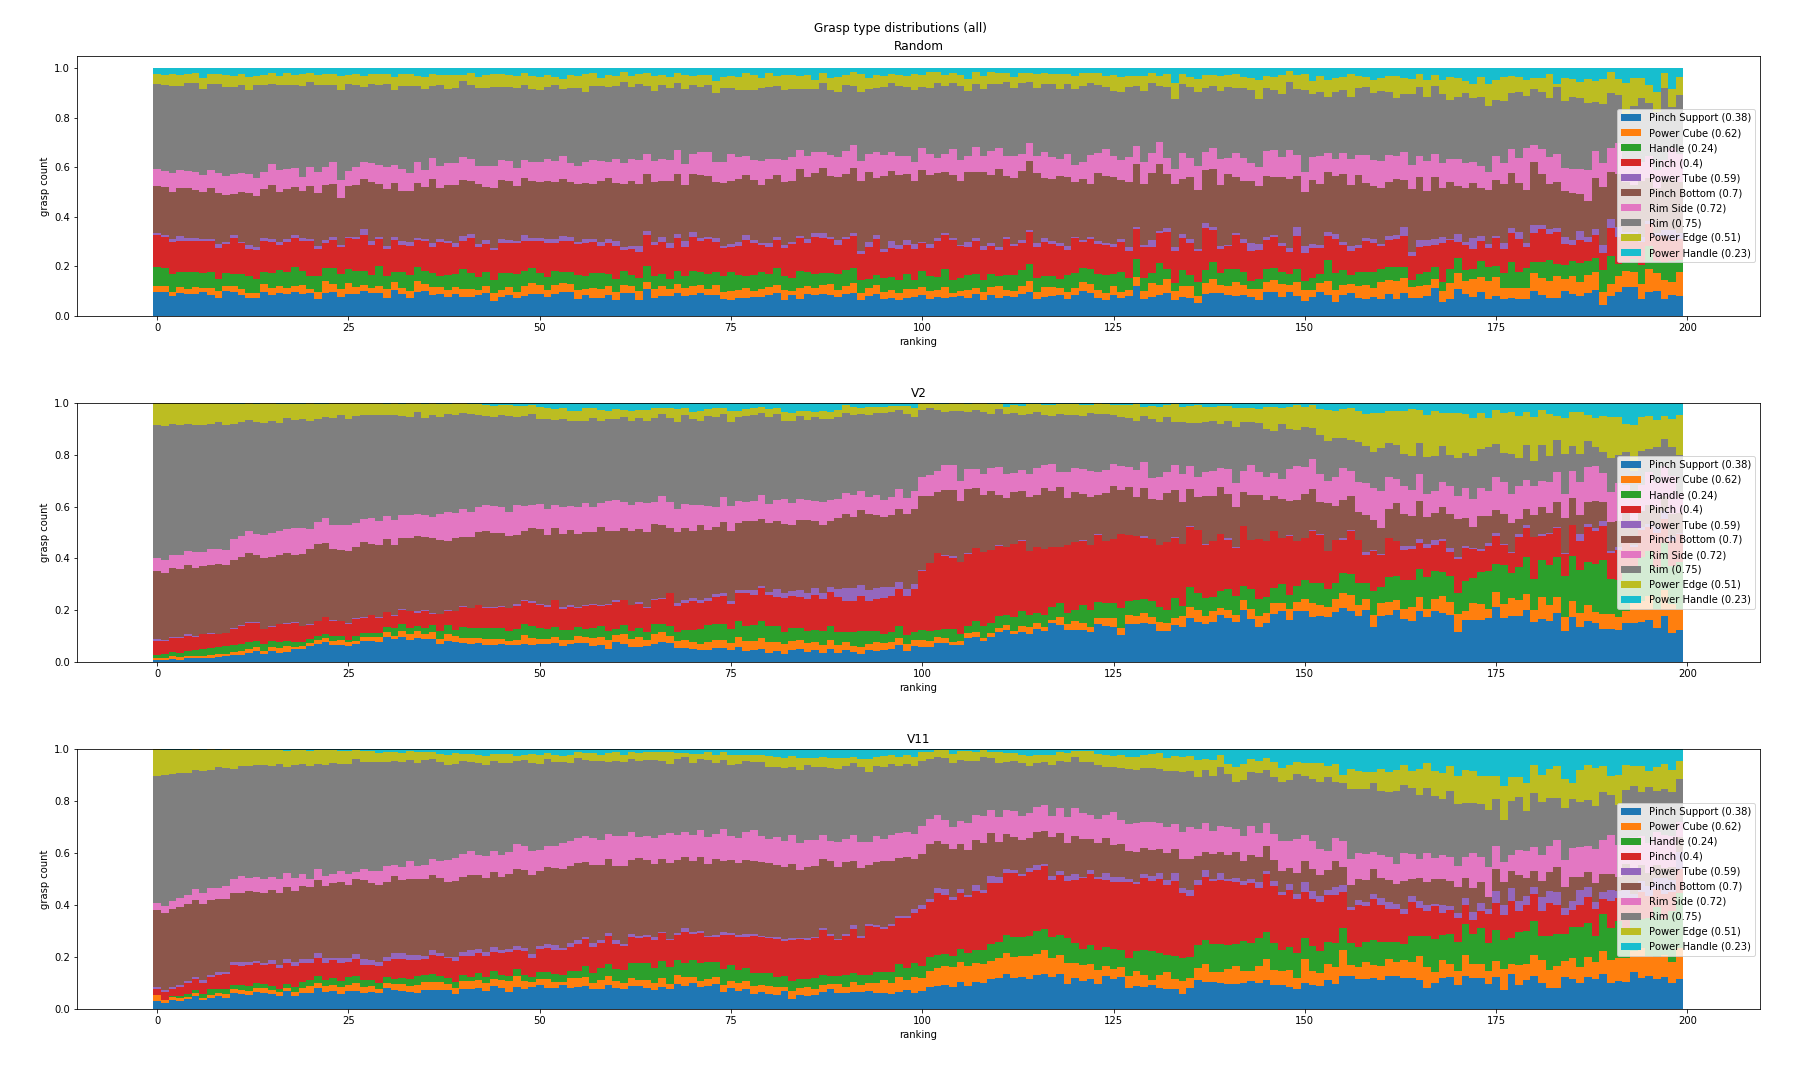
\includegraphics[width=0.8\columnwidth]{images/post-analysis/[6] Grasp_type_distributions_all.png}
\caption{Comparison of grasp type distributions per ranking of random ranking,V2 and V11.}
\label{fig:post6}
\end{figure}

\begin{figure}
\centering
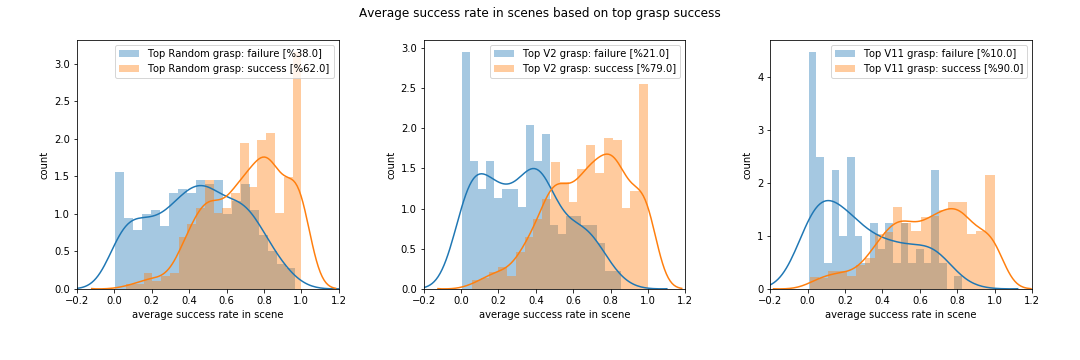
\includegraphics[width=0.8\columnwidth]{images/post-analysis/[7] Average_success_rate_in_scenes_based_on_top_grasp_success.png}
\caption{Average success rate in scenes vs top grasp success.}
\label{fig:post7}
\end{figure}

\begin{figure}
\centering
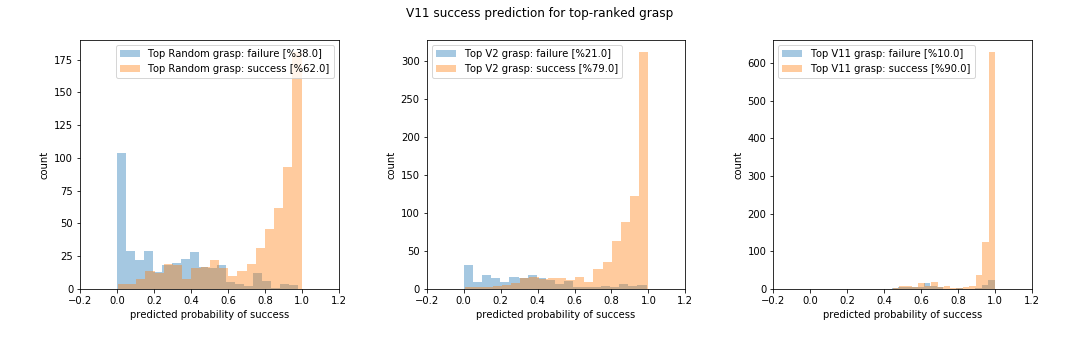
\includegraphics[width=0.8\columnwidth]{images/post-analysis/[8] V11_success_prediction_for_top-ranked_grasp.png}
\caption{Histogram of success rate of a top-ranked grasp vs its probability of success as estimated by V11.}
\label{fig:post8}
\end{figure}

\begin{figure}
\centering
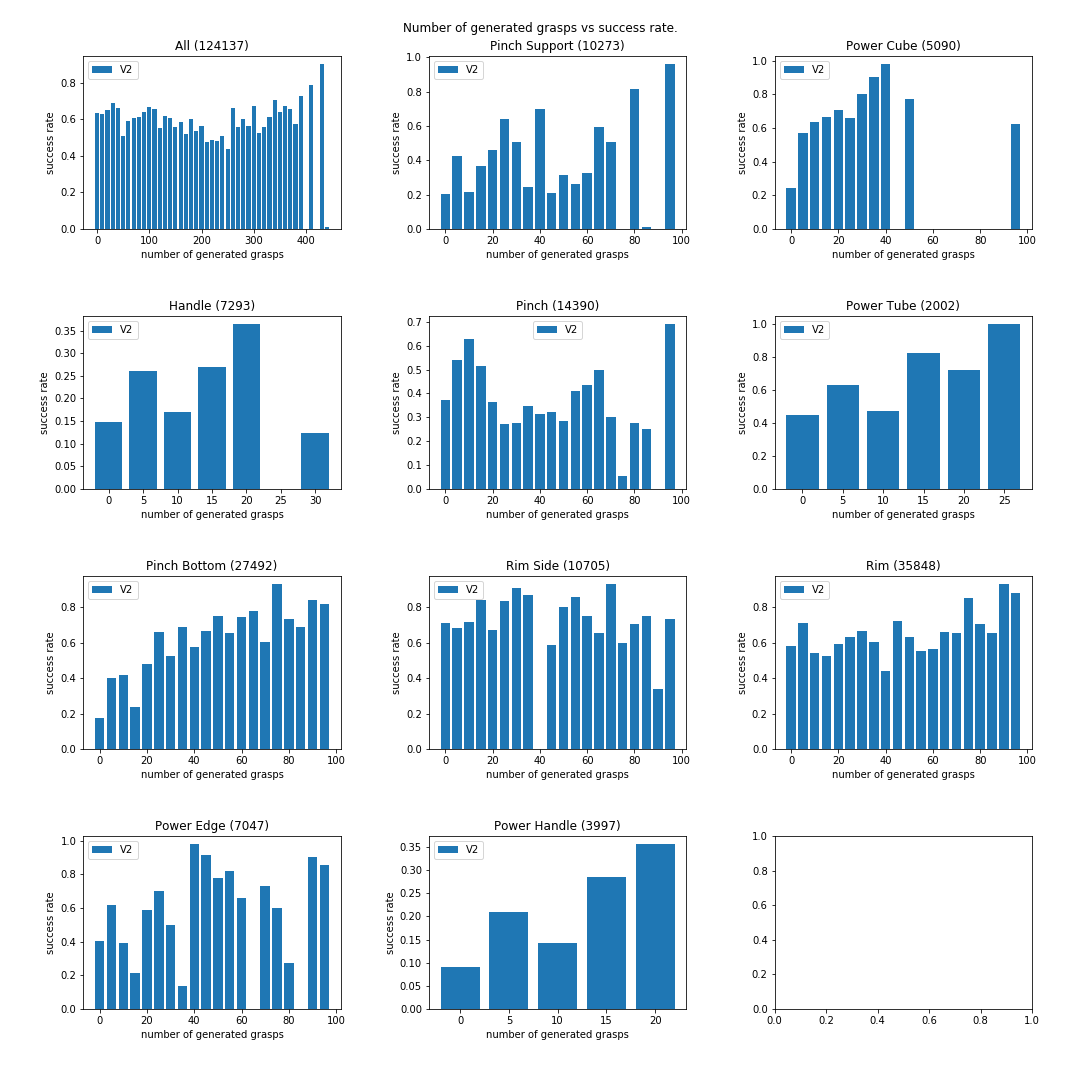
\includegraphics[width=0.8\columnwidth]{images/post-analysis/[10] number_of_generated_grasps_vs_success_rate.png}
\caption{Correlation of success rate with number of generated grasps per scene per grasp type.}
\label{fig:post10}
\end{figure}

\begin{figure}
\centering
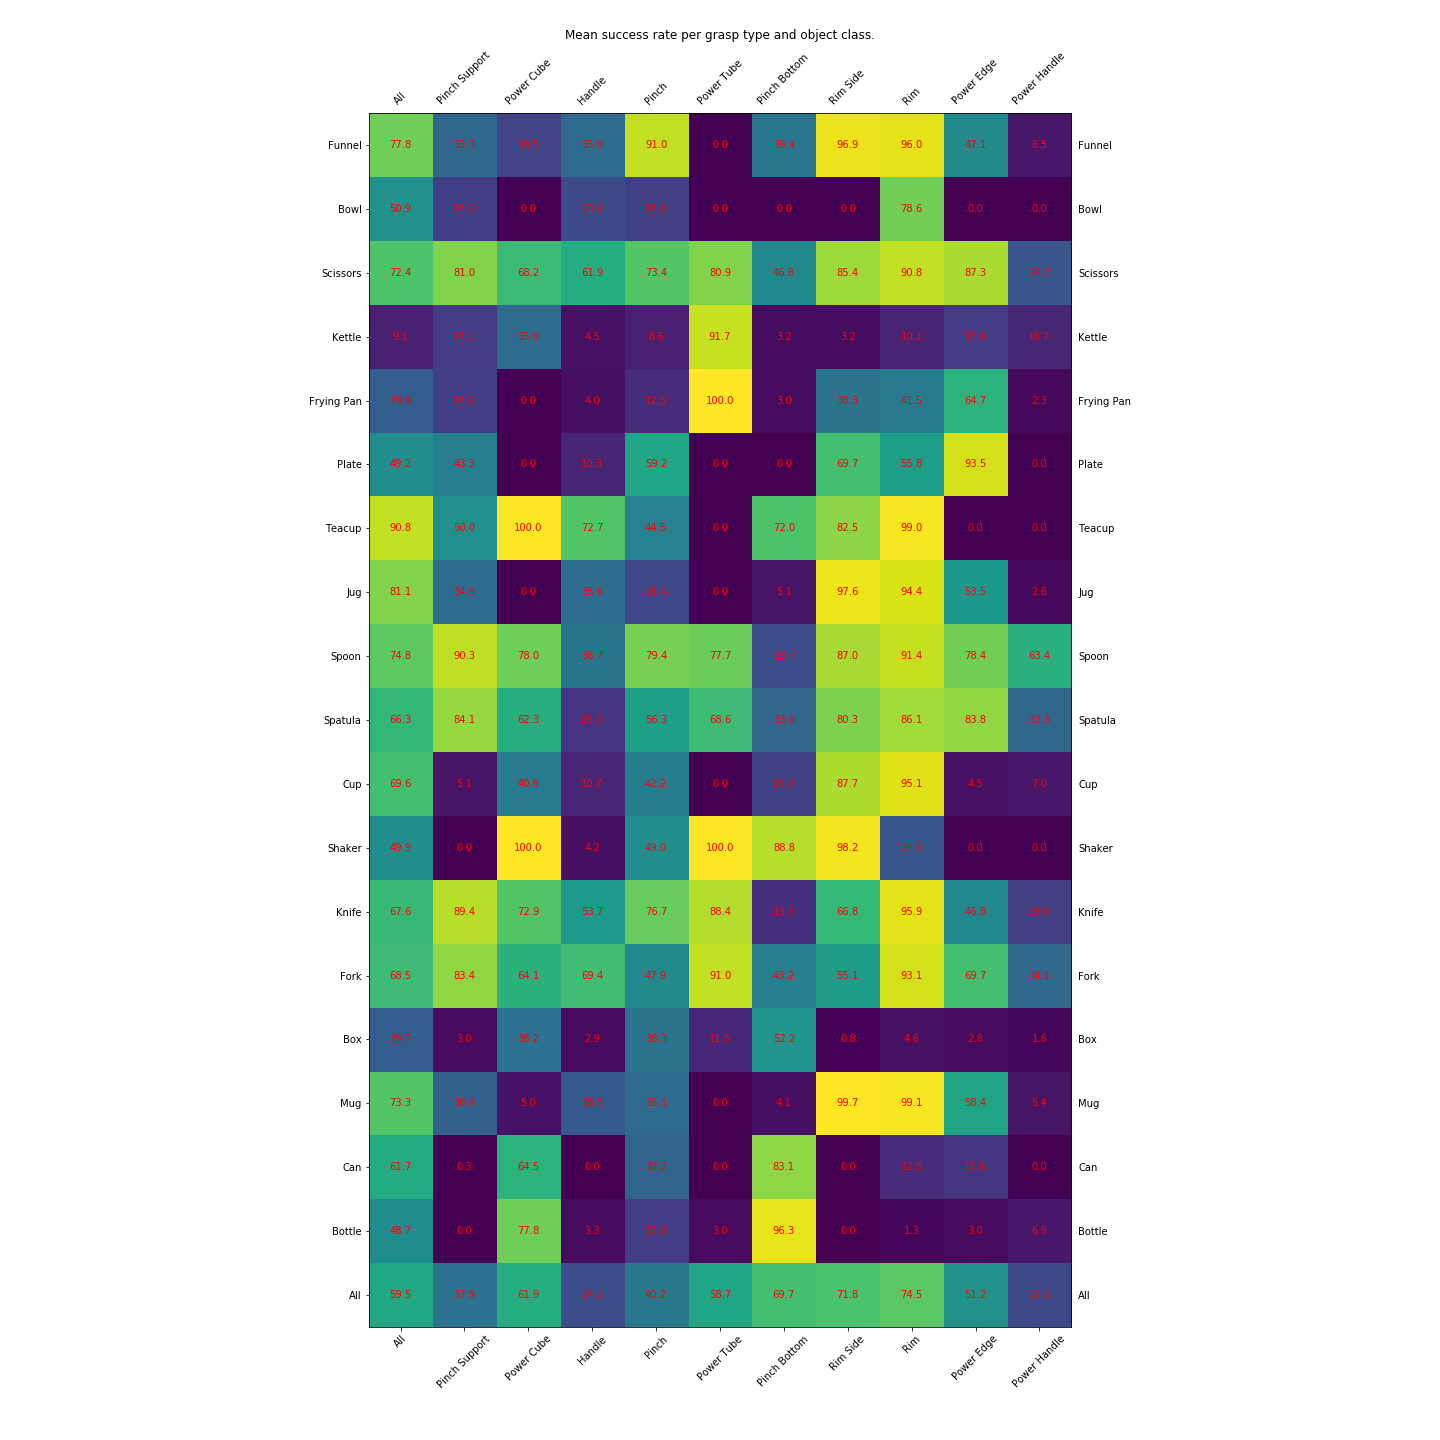
\includegraphics[width=0.8\columnwidth]{images/post-analysis/[12] mean_success_rate_per_grasp_type_and_object_class.png}
\caption{Mean success rate per grasp type and object class.}
\label{fig:post12}
\end{figure}

\begin{figure}
\centering
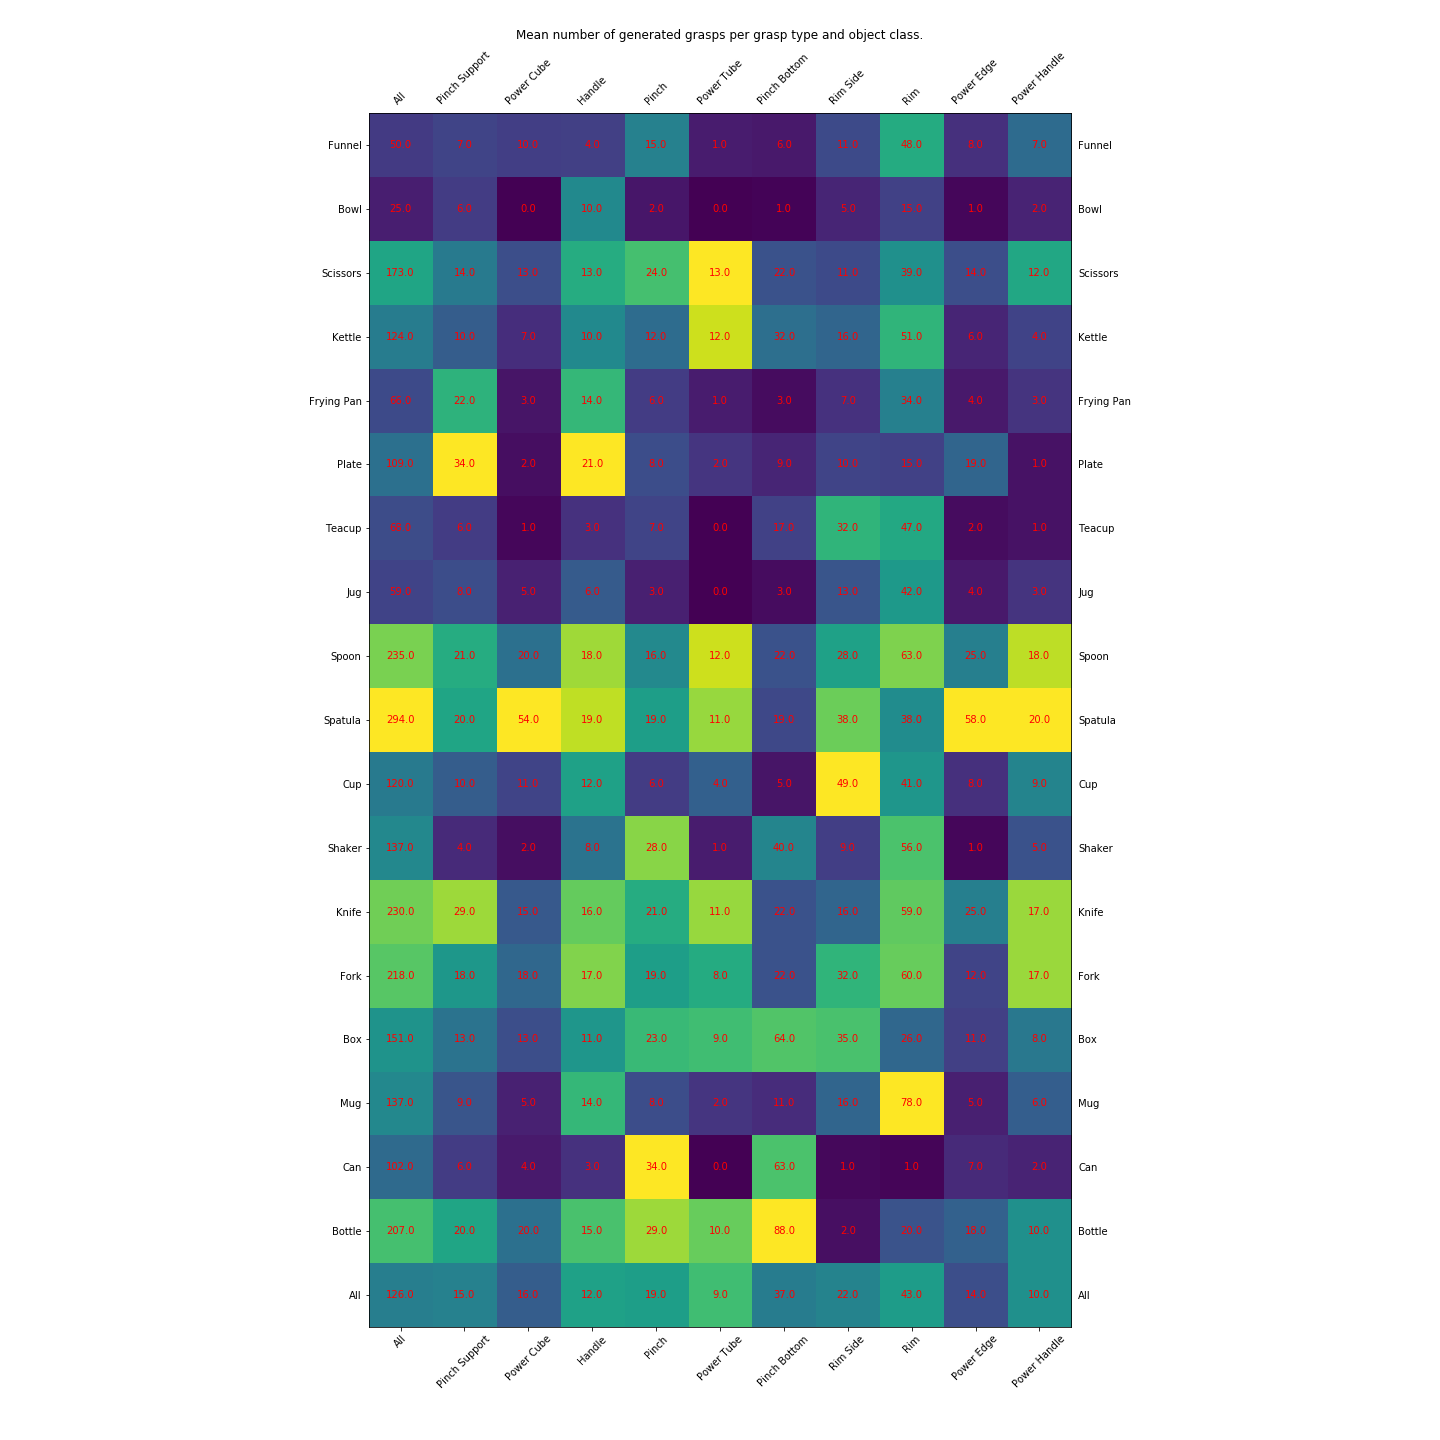
\includegraphics[width=0.8\columnwidth]{images/post-analysis/[13] mean_number_of_generated_grasps_per_grasp_type_and_object_class.png}
\caption{Mean number of generated grasps per grasp type and object class.}
\label{fig:post13}
\end{figure}


%We compared the EM and GM rankings (Figure~\ref{fig:successvsranking}). The x-axis shows the ranking. The y-axis shows the average actual success rate over all scenes (1,241 test, 7,311 training). When ranked by the EM, the grasp success probability falls nearly monotonically, as is desirable. On the other hand, the likelihood-based ranking of GM results in many good grasps being low-ranked. We also wish to know whether the grasps recommended by the EM and the GM have different grasp success rates. The success rates of the top-ranked grasps are 71.59\% (GM) and  84.2\% (EM).

%A pure generative model architecture (GM) and the generative-evaluative architecture (GEA) were evaluated using a paired trials methodology. Each was presented with the same object-pose combinations. Each architecture generated a ranked list of grasps, and the highest ranked grasp was executed. The highest-ranked grasp based on the predicted success probability of the network is performed on each scene. A grasp was deemed successful if, when lifted for five seconds, the object then remained stable in the hand for a further five seconds before being automatically released. The success rate for GM was 57.1\% and for GEA it was 77.6\%. The successes and failures for each method were recorded and are summarised in Table~\ref{tab:robot-results}. A two-tailed McNemar test, for the difference between success rates for paired comparison data, was performed and the difference between the two algorithms has a $p$-value of 0.0442, and so is statistically significant. A selection of grasps where the two methods performed differently are shown in Figure~\ref{fig:successfail}.

% OLD TABLE
%\begin{table}
%\begin{center}
%\caption{Results of the real robot paired comparison trial.}
%\begin{tabular}{|c|c|c|c|}  \hline 
%          &                & \multicolumn{2}{ c |}{ GM} \\ \hline
%          &                & \# succs & \# fails  \\  \hline
 %GEA  & \# succs &  23 &  15  \\
 %         & \# fails    &  5   &   6   \\ \hline
%\end{tabular}
%\end{center}
%\label{tab:robot-results}
%\end{table}

%Training parameters for network. Training of example grasps for learning from demonstration. Creation of real test data set. Paired comparisons methodology with vanilla LFD algorithm (pose + object + camera view).
%
%The actual grasping tests have been performed on the real robot. 